\chapter{Solution}
\label{cha:solution}
The solution to the problem will be demonstrated with an example page using a selection of demo components that will test the functionality of all the concepts described in the Fundamentals and Related Works chapter.
\section{Compiling Stencil Components}
Stencil offers two ways of compiling its components into a format that can be used by other frameworks. The first way is to compile a component into a pure JavaScript file. The second way is to use the Stencil compiler's output target feature which can compile a Stencil component into a framework native component.

\subsection{Pure JavaScript}
The easy and less time consuming way of compiling a Stencil component is to compile it into a standardized JavaScript web component. These component is then ready for any browser to interpret. However if used in a framework, a small amount of boiler plate code is necessary in each of the frameworks.\\[0.5cm]
%
The picture below shows the demo components that will be used as an example. 
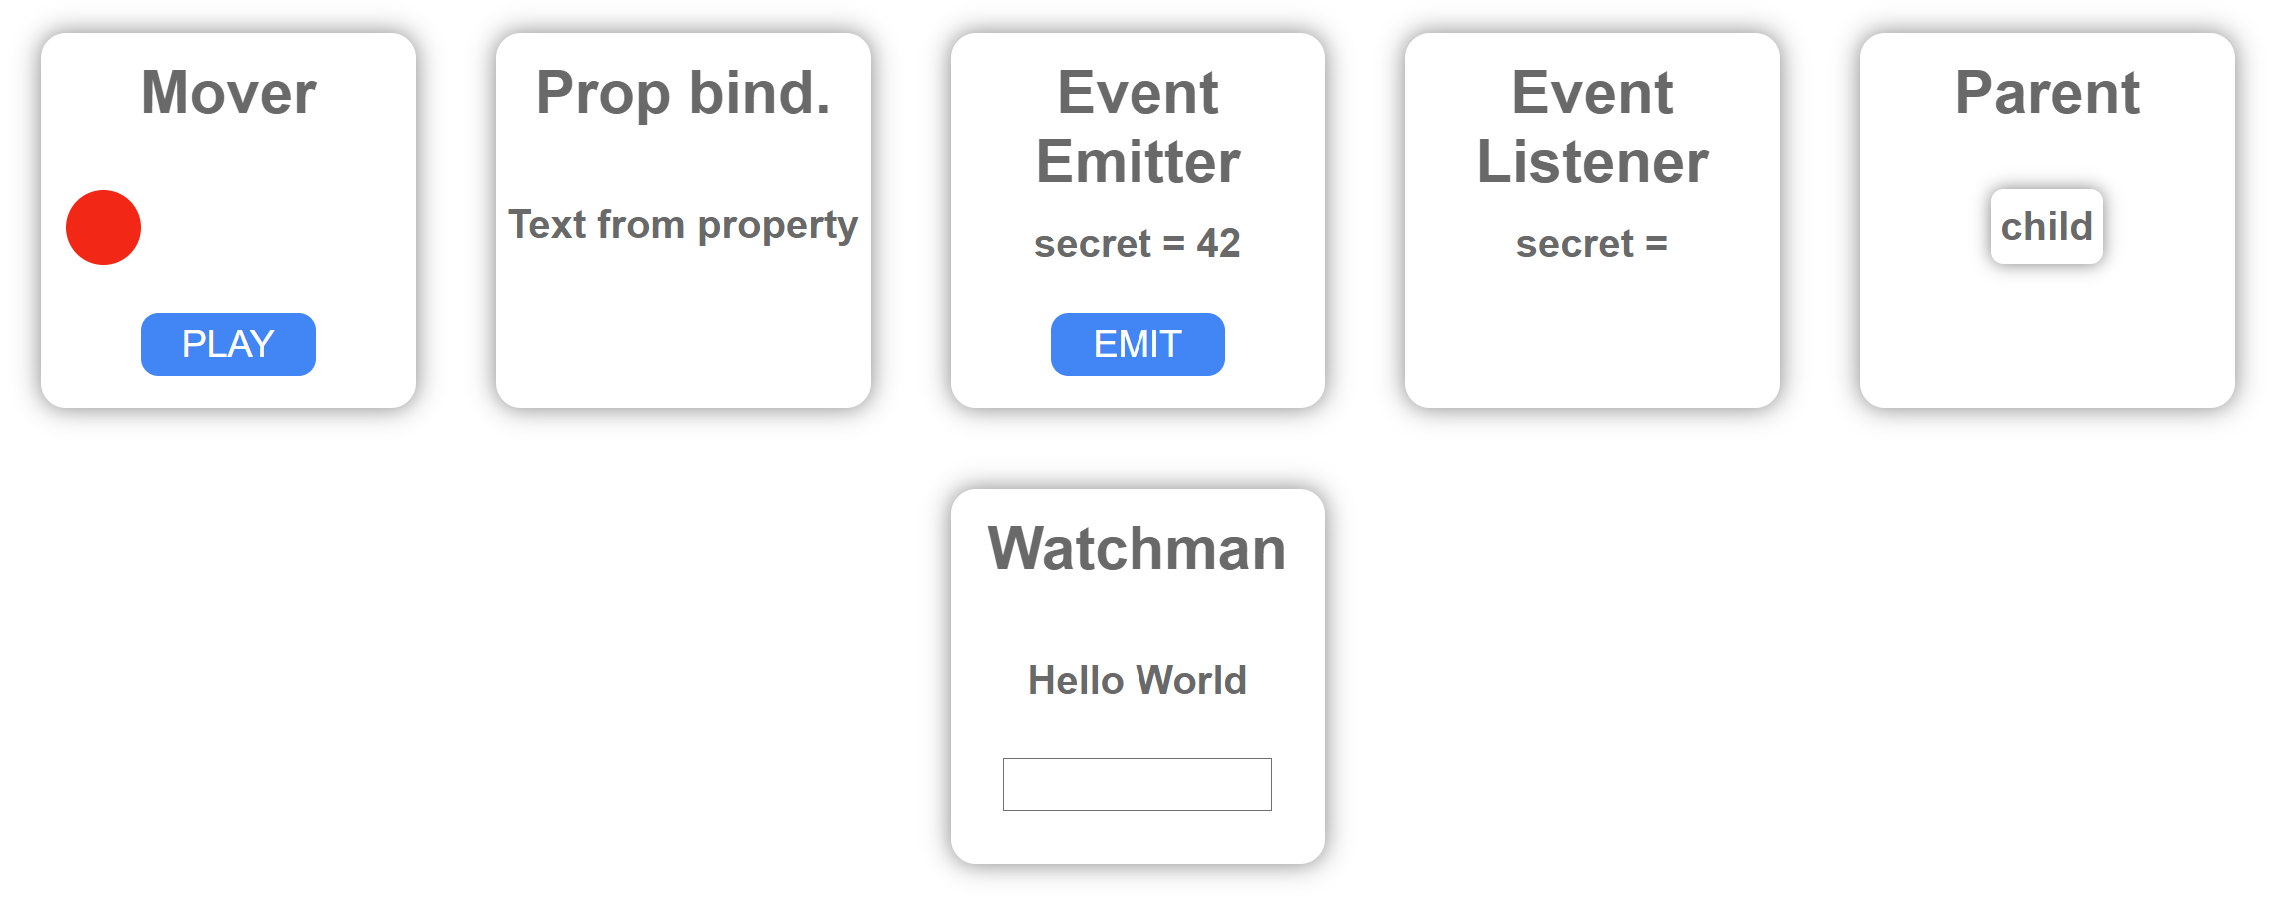
\includegraphics [height=6.2cm, width=15cm] {images/demopage}
About these components:
\begin{itemize}
\item \textbf{Mover:} A bare bones hello world component that plays a little CSS animation to test whether components and styling are displayed properly.
\item \textbf{Property binding:} This component uses a prop decorator to receive text via HTML to test the functionality of property binding.
\item \textbf{Event Emitter:} This component has a secret value in its class and uses an event decorator to emit a DOM event containing this secret which can be processed by other components.
\item \textbf{Event Listener:} Uses a listen decorator to catch the event emitted by the event emitter component and display the secret in its own template.
\item \textbf{Parent and Child:} The Parent component contains a child component which is displayed in its template to test component nesting.
\item \textbf{Watchman:} The watchman component uses a watch decorator to watch its state, a string variable, for changes. Through user input via textbox this state is changed with every keystroke and the displayed text will change along with the state. This component tests the event binding and its equivalents in React and Vue.
\end{itemize}
A component library created in Stencil can be compiled using the console command \verb+npm run build+.\\
This script will start the compiler, which then creates a directory named "dist". This directory contains a components directory that holds the resulting framework agnostic components. Along with these components, the dist directory also contains numerous JavaScript resources, which frameworks need for various loading or importing purposes.

\subsection{Output Targets}
Stencil's output targets feature allows users to compile stencil components into framework native components. This makes it easier to make changes when consuming a component.
\subsubsection{Angular}

